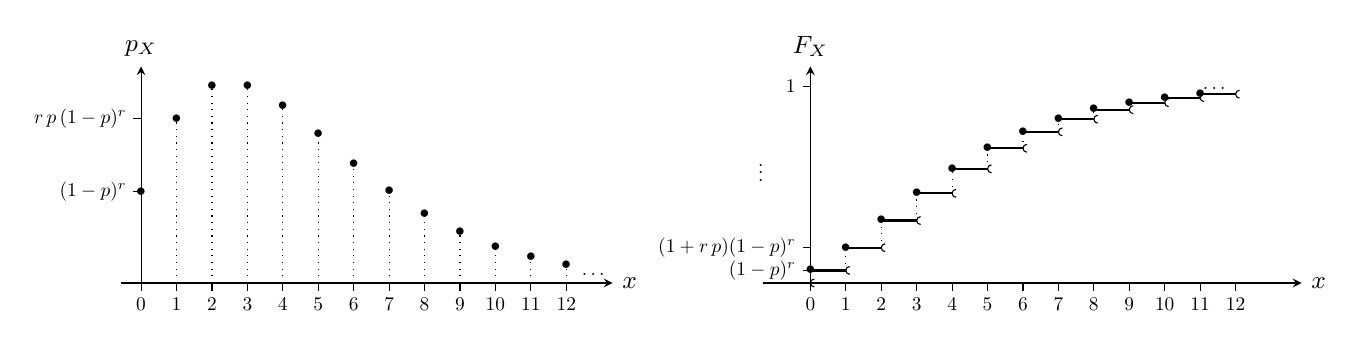
\begin{tikzpicture}%[scale=.9]
\shorthandoff{>}
%
\pgfmathsetmacro{\sx}{.45};% x-scaling
\pgfmathsetmacro{\r}{.05};% radius arc non continuity F_X
\pgfmathsetmacro{\p}{3/5};% probabilidad p de suceso
\pgfmathsetmacro{\rp}{3};% numero r de fracascos
\pgfmathsetmacro{\n}{12};% numero maximo a dibujar
\pgfmathsetmacro{\q}{max(floor((\rp-1)*\p/(1-\p)),0)};% modo de la binomial negativa
\pgfmathsetmacro{\m}{factorial(\q+\rp-1)*((1-\p)^\rp)*(\p^\q)/factorial(\rp-1)/factorial(\q)};
%{factorial(\n)/factorial(\q)/factorial(\n-\q)*(\p^\q)*((1-\p)^(\n-\q))};% maximo de la binomial
% masa
\begin{scope}
%
\pgfmathsetmacro{\sy}{2.5/\m};% y-scaling 
\draw[>=stealth,->] (-.25,0)--({\sx*(\n+.75)+.25},0) node[right]{\small $x$};
\draw[>=stealth,->] (0,-.1)--(0,{\sy*\m+.25}) node[above]{\small $p_X$};
%
\pgfmathsetmacro{\b}{(1-\p)^\rp};% coeficiente binomial por la probabilidad
%
\foreach \k in {0,...,\n} {
\draw ({\k*\sx},0)--({\k*\sx},-.1) node[below,scale=.7]{$\k$};
\draw[dotted] ({\k*\sx},0)--({\k*\sx},{\sy*\b}) node[scale=.7]{$\bullet$};
%
\pgfmathsetmacro{\bl}{\b*\p*(\k+\rp)/(\k+1)};\global\let\b\bl;% proba actualizada
}
\draw ({(\n+.25)*\sx},{\sy*\b*(\n+1)/\p/(\n+\rp)/2}) node[right,scale=.7]{\ldots};
\draw (0,{((1-\p)^\rp)*\sy})--(-.1,{((1-\p)^\rp)*\sy}) node[left,scale=.7]{$(1-p)^r$};
\draw (0,{\rp*\p*((1-\p)^\rp)*\sy})--(-.1,{\rp*\p*((1-\p)^\rp)*\sy}) node[left,scale=.7]{$r \, p \, (1-p)^r$};
%\draw (0,{(\rp*\p*((1-\p)^\rp)+\m)/2*\sy}) node[scale=.7]{$r \, p \, (1-p)^r$};
%
\end{scope}
%
%
% reparticion
\begin{scope}[xshift=8.5cm]
%
\pgfmathsetmacro{\sy}{2.5};% y-scaling 
%
\draw[>=stealth,->] (-.6,0)--({\sx*(\n+.75)+.5},0) node[right]{\small $x$};
\draw[>=stealth,->] (0,-.1)--(0,{\sy+.25}) node[above]{\small $F_X$};
%
\pgfmathsetmacro{\b}{(1-\p)^\rp};% coeficiente binomial por la probabilidad
\pgfmathsetmacro{\c}{(1-\p)^\rp};% cumulativa binomial por la probabilidad
%
% cumulativa x < 0
\draw (0,0)--(0,-.1) node[below,scale=.7]{$0$};
\draw[thick] (-.5,0)--(0,0);
\draw (\r,\r) arc (90:270:\r);
%
% cumulativa x de 0 a n-1
\foreach \k in {1,...,\n} {
\draw ({\k*\sx},0)--({\k*\sx},-.1) node[below,scale=.7]{$\k$};
\draw[thick]({(\k-1)*\sx},{\sy*\c}) node[scale=.7]{$\bullet$}--({\k*\sx},{\sy*\c});
\draw ({\k*\sx+\r},{\sy*\c+\r}) arc (90:270:\r);
\draw[dotted] ({(\k-1)*\sx},{(\c-\b)*\sy})--({(\k-1)*\sx},{\c*\sy});
%
\pgfmathsetmacro{\bl}{\b*\p*(\k+\rp-1)/\k};\global\let\b\bl;% proba actualizada
\pgfmathsetmacro{\cl}{\c+\b};\global\let\c\cl;% cumulativa actualizada
}
%
\draw ({\n*\sx},{\sy*(\c+1)/2}) node[left,scale=.7]{\ldots};
\draw (0,{((1-\p)^\rp)*\sy})--(-.1,{((1-\p)^\rp)*\sy}) node[left,scale=.7]{$(1-p)^r$};
\draw (0,{(1+\rp*\p)*((1-\p)^\rp)*\sy})--(-.1,{(1+\rp*\p)*((1-\p)^\rp)*\sy}) node[left,scale=.7]{$(1+r \, p) (1-p)^r$};
\draw (-.75,{((1+\rp*\p)*((1-\p)^\rp)+1)/2*\sy}) node[right,scale=.7]{$\vdots$};
\draw (0,\sy)--(-.1,\sy) node[left,scale=.7]{$1$};
\end{scope}
%
\end{tikzpicture}